\documentclass[11pt]{article}
\usepackage[a4paper,margin=1in]{geometry}
\usepackage{amsmath,amssymb}
\usepackage{booktabs}
\usepackage{graphicx}
\usepackage{caption}
\usepackage{xcolor}
\usepackage{needspace}
\usepackage[colorlinks=true,linkcolor=blue!50!black,citecolor=blue!50!black,urlcolor=blue!50!black]{hyperref}
\graphicspath{{../../figures/}}
% generated by scripts/make_paper_tables.py from results/; do not edit
\newcommand{\armARatio}{1.505}
\newcommand{\armBRatio}{0.978}
\newcommand{\armBRemoved}{63}
\newcommand{\lamCorr}{4.7}
\newcommand{\lamGnn}{2.2}
\newcommand{\lamNaive}{3.7}
\newcommand{\nineBErrors}{1\,079}
\newcommand{\nineBShots}{700\,000}
\newcommand{\nineErrors}{1\,076}
\newcommand{\nineRatio}{1.46}
\newcommand{\nineRemoved}{88}
\newcommand{\nineShots}{700\,000}
\newcommand{\precMax}{0.967}
\newcommand{\precMin}{0.925}
\newcommand{\recMax}{0.88}
\newcommand{\recMin}{0.77}
\newcommand{\slowMax}{31}
\newcommand{\slowMin}{23}
\newcommand{\thrNaive}{0.83}
\newcommand{\warmGain}{15}

\captionsetup{font=small,labelfont=bf}
\setlength{\parskip}{0.4em}
\setlength{\parindent}{0pt}

\title{When does a neural decoder help? Graph neural network decoders and a neural pre-decoder\\
against minimum-weight matching for the surface code under mismatched circuit noise}
\author{Uhenraj Jarga Magar\\ \small Draft, \today}
\date{}

\begin{document}
\maketitle

\begin{abstract}
Minimum-weight perfect matching (MWPM) is the standard surface-code decoder, but it is only as good as the noise model it is given. We ask when a neural decoder trained on syndromes alone can beat it. We benchmark a graph neural network (GNN) over fired detectors against naive, calibrated, oracle and correlated matching on rotated surface-code memory experiments ($d=3,5,7$) under SI1000 circuit noise with per-qubit heterogeneity, bad couplers, drift and crosstalk, using identical shots for every decoder. The GNN ties or beats matching at $d=3$ and, under crosstalk, at $d=5$, but is about twice as bad at $d=7$, does not transfer from smaller distances, and needs about $100\times$ more data than calibrated matching; mismatch alone gives matching little to lose. We then study a local neural pre-decoder that removes isolated faults, identified with fault-level labels from Stim's sampler, before matching. Evaluated under a pre-registered protocol, it improves on matching at the distances it was trained on, but at $d=7$ the validation-chosen threshold fails the pre-registered criterion (\nineRatio$\times$ matching's logical error rate at $p=0.002$). A stricter threshold was then confirmed on fresh shots: ratio \armBRatio{} while removing \armBRemoved\% of fired detectors. A matching-graph pitfall (lost logical labels on parallel edges) and the cost of the Python implementation are also reported. All code, results and run records are in the accompanying repository.
\end{abstract}

\section{Introduction}
Quantum error correction decodes a stream of parity-check outcomes (a \emph{syndrome}) into a guess of which logical error occurred. Minimum-weight perfect matching~\cite{dennis2002,fowler2015} is fast and accurate when faults are independent and graph-like, and modern implementations~\cite{higgott2022,higgott2023sparse} scale to very large codes. Its weakness is twofold: it must split correlated faults, such as a $Y$ error that flips both $X$- and $Z$-type detectors, into independent edges, and its edge weights come from a noise model that may not match the device. Neural decoders learn a direct map from syndrome to logical outcome and so can, in principle, absorb both effects; recent work shows large gains on hardware-scale experiments~\cite{bausch2024} and for graph-based architectures~\cite{lange2025}.

Claims of neural advantage are only meaningful against strong, fairly constructed baselines. This paper is a benchmark designed with that in mind. We ask three questions: (i) when the true noise differs from matching's model, does a syndrome-only neural decoder gain over \emph{naive}, \emph{calibrated} (weights re-estimated from syndrome data) and \emph{oracle} matching? (ii) Does it keep its advantage as the code distance grows? (iii) Can a neural component be combined with matching so that matching's scaling is retained?

\Needspace{9\baselineskip}
\textbf{Contributions.}
\begin{itemize}
\item A reproducible benchmark with per-qubit and per-gate noise, five noise scenarios and six matching baselines, in which every decoder sees the same sampled shots, with multi-seed statistics and paired tests.
\item Evidence that, in this setting, mismatch gives matching little to lose (calibration recovers essentially all of it), that a distance-agnostic GNN does not scale to $d=7$, and that warm-starting from smaller distances helps only modestly.
\item A neural pre-decoder trained on fault-level labels, evaluated under a pre-registered decision rule and a pre-registered confirmatory test on fresh shots, including the honest report that the first threshold failed and a stricter one was needed.
\item A practical pitfall: when several fault mechanisms share a detector pair but differ in their logical effect, a matching graph keeps only one logical label, which can silently handicap the ``oracle'' baseline.
\end{itemize}

\section{Background and related work}
\textbf{Surface code and decoding.} A stabiliser code is defined by a binary parity-check matrix $H$; errors $e\in\mathbb F_2^n$ yield the syndrome $s=He \bmod 2$, and decoding chooses a correction consistent with $s$ that preserves the logical state. For the surface code~\cite{fowler2012} under circuit noise, each single fault flips at most two detectors of a given type, so the detector error model can be turned into a weighted graph with edge weights $\log\frac{1-p}{p}$, and the most likely error is a minimum-weight perfect matching of the fired detectors. Faults that flip more detectors are split into graph-like pieces, discarding their correlation; PyMatching~\cite{higgott2022,higgott2023sparse} additionally offers a two-pass correlated mode, and belief matching~\cite{higgott2023belief} reweights edges using belief propagation.

\textbf{Neural decoders.} Early neural decoders targeted small codes~\cite{torlai2017}; recurrent-transformer decoders trained on large simulated datasets and fine-tuned on hardware data have reported lower logical error rates than matching-based decoders~\cite{bausch2024}, and graph neural networks over fired detectors offer distance-independent weights~\cite{lange2025}. Neural components have also been used \emph{locally}, to reduce the load on a global decoder~\cite{delfosse2020,chamberland2023}; our pre-decoder follows that idea.

\section{Methods}
\subsection{Circuits and noise}
We simulate rotated surface-code memory experiments (Z basis, $\text{rounds}=d$, $d\in\{3,5,7\}$) with Stim~\cite{gidney2021stim}. The base noise is SI1000~\cite{gidney2021honeycomb}: two-qubit gates depolarise at rate $p$, single-qubit gates and idling at $p/10$, resets flip at $2p$, measurements at $5p$ (idling qubits during measurement and reset at $2p$). Noise is inserted by our own pass so that every qubit and gate can carry its own rate; with uniform rates it reproduces Stim's generated noise exactly (unit-tested). Logical error rates are reported per round, $\epsilon=\tfrac12\bigl(1-(1-2P_L)^{1/r}\bigr)$. With naive matching the $d=5$ and $d=7$ curves cross at $p\approx\thrNaive\%$.

\begin{table}[t]
\centering\small
\begin{tabular}{@{}lp{0.8\linewidth}@{}}
\toprule
Scenario & True noise \\
\midrule
S0 & uniform SI1000 (control) \\
S1 & every qubit/gate rate $\times e^{0.5z}$, $z\sim\mathcal N(0,1)$, channel means preserved \\
S2 & S1 plus three random CX gates at $8\times$ their rate \\
S3 & S2 at calibration time; at test time every rate additionally $\times e^{0.3z'}$ (drift) \\
S4 & SI1000 plus correlated $XX$ and $ZZ$ faults at $0.25p$ between neighbouring data qubits in different CX gates of a layer \\
\bottomrule
\end{tabular}
\caption{Noise scenarios. A \emph{device instance} is one seeded draw of the rates; S1--S3 are averaged over three instances. S4's strength was lowered from $1.0p$ to $0.25p$ because at $1.0p$ error rates grew with $d$ (above threshold).}
\label{tab:scenarios}
\end{table}

\subsection{Decoders}
All matching decoders use PyMatching on a detector error model (DEM). \textbf{Naive} uses the nominal SI1000 model at $p$; \textbf{calibrated} re-estimates edge probabilities from detection-event correlations on $10^6$ shots of the device (the standard $p_{ij}$ estimator); \textbf{oracle} uses the exact true model; \textbf{correlated} and \textbf{oracle correlated} use PyMatching's correlated mode on the naive and true models. The \textbf{GNN} sees only syndromes and logical labels.

\subsection{GNN decoder}
Nodes are the \emph{fired detectors} only, with distance-independent features (stabiliser type, distances to the four lattice boundaries in raw lattice units clipped at 4, and first/last-round flags). Edges join the 8 nearest neighbours in space-time. Four message-passing layers (hidden width 64, residual connections, LayerNorm) are followed by mean and max pooling and an MLP head giving the logical-flip logit; the model has 133,761 parameters, is written in plain PyTorch, and runs unchanged at any distance. Shots are sampled on the fly across a band of error rates and the model is trained with Adam and cosine decay for 12\,000 steps of 1\,024 shots ($\approx12$M shots), with early stopping on a fixed validation set disjoint from the test shots.

\subsection{Neural pre-decoder}
A fault is \emph{isolated} in a shot if it fired and no other fired fault touches either of its detectors; it is then the unambiguous explanation of those detectors. Stim's detector-error-model sampler returns, for each shot, which fault mechanisms fired, which gives exact labels. The pre-decoder is a GNN of the same body as above with two heads: a symmetric pair head scoring each \emph{pair candidate} (a pair of fired detectors that is an edge of the matching graph) and a boundary head scoring each fired detector with a boundary edge, trained with binary cross-entropy to predict ``isolated''. At inference, candidates scored at least $\tau$ are removed, greedily by probability so that no detector is used twice; the logical labels of the removed faults are accumulated, and the residual syndrome is decoded by the \emph{same} matching graph and weights as the baseline. The prediction is matching's output XOR the removed faults' logical effect. Three models are trained on $d=3,5$ jointly and one reference at $d=7$, with the GNN recipe above.

\subsection{Evaluation protocol}
\textbf{Identical shots.} For each point, all decoders decode the same sampled syndromes, sampled until the reference decoder has seen at least 100 logical errors (1\,000 at the key $d=7$, $p=0.002$ point of the pre-decoder study); Wilson 95\% intervals and, where per-shot results are stored, exact McNemar tests on the discordant shots are reported. Seed ranges for training, validation and test never overlap (unit-tested). \textbf{Statistics.} GNNs use three training seeds; S1--S3 use three device instances; $\pm$ is a standard deviation over seeds or instances as stated.

\textbf{Pre-registration.} For the pre-decoder, the threshold $\tau$ was chosen on $d=5$ \emph{validation} shots only and applied unchanged at every distance; the success criterion was fixed before any test shot: \emph{positive} if at $d=7$ zero-shot, $p=0.002$, the logical error rate is at most $1.05\times$ matching's \emph{and} at least $30\%$ of fired detectors are removed. A confirmatory test on fresh shots followed, with its rule and a later amendment written down and committed before any of its shots were run (Section~\ref{sec:confirm}).

\section{Results}
\subsection{Uniform noise}
\begin{figure}[t]
\centering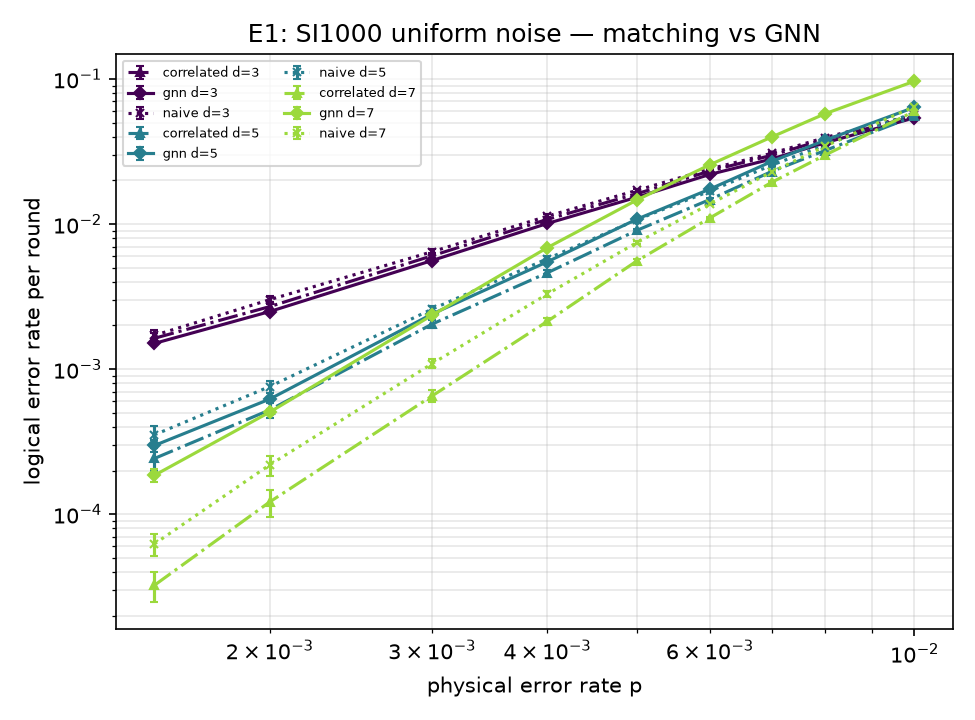
\includegraphics[width=0.72\linewidth]{e1_clean.png}
\caption{Per-round logical error rate under uniform SI1000 noise (S0) for naive matching, correlated matching and the GNN. The GNN is lowest at $d=3$ and falls behind as $d$ grows.}
\label{fig:e1}
\end{figure}
\begin{table}[t]
\centering\small
\begin{tabular}{lccc}
\toprule
Decoder & $d=3$ & $d=5$ & $d=7$ \\
\midrule
naive MWPM & $3.01\times10^{-3}$ & $7.58\times10^{-4}$ & $2.19\times10^{-4}$ \\
calibrated MWPM & $2.95\times10^{-3}$ & $7.40\times10^{-4}$ & $2.10\times10^{-4}$ \\
correlated MWPM & $2.70\times10^{-3}$ & $5.23\times10^{-4}$ & $1.22\times10^{-4}$ \\
GNN (3 seeds) & $(2.49\,\pm\,0.01)\times10^{-3}$ & $(6.22\,\pm\,0.05)\times10^{-4}$ & $(5.05\,\pm\,0.23)\times10^{-4}$ \\
\bottomrule
\end{tabular}

\caption{S0, $p=0.002$: per-round logical error rate (GNN: mean $\pm$ std over three seeds). Naive, calibrated and oracle matching coincide under uniform noise; correlated matching equals its oracle version.}
\label{tab:e1}
\end{table}
Under uniform noise (Table~\ref{tab:e1}, Fig.~\ref{fig:e1}) the GNN is the best decoder at $d=3$, ahead of naive and calibrated matching by a clear margin and of correlated matching by a small one (per-shot error $0.0075$ vs $0.0080$ at $p=0.002$, with overlapping intervals). It sits between naive and correlated matching at $d=5$ and is far behind at $d=7$. The error-suppression factor per distance step ($\epsilon\propto\Lambda^{-(d+1)/2}$) at $p=0.002$ is $\Lambda\approx\lamNaive$ for naive matching, $\lamCorr$ for correlated matching and only $\lamGnn$ for the GNN.

\subsection{Mismatched noise}
\begin{table}[t]
\centering\small
\begin{tabular}{lccc}
\toprule
Decoder & $d=3$ & $d=5$ & $d=7$ \\
\midrule
naive MWPM & $1.20\times10^{-2}$ & $6.08\times10^{-3}$ & $3.16\times10^{-3}$ \\
calibrated MWPM & $1.15\times10^{-2}$ & $5.48\times10^{-3}$ & $2.79\times10^{-3}$ \\
oracle MWPM & $1.20\times10^{-2}$ & $5.54\times10^{-3}$ & $2.86\times10^{-3}$ \\
correlated MWPM & $1.12\times10^{-2}$ & $4.98\times10^{-3}$ & $2.17\times10^{-3}$ \\
oracle correlated MWPM & $1.11\times10^{-2}$ & $4.44\times10^{-3}$ & $1.89\times10^{-3}$ \\
GNN & $1.02\times10^{-2}$ & $5.46\times10^{-3}$ & $6.35\times10^{-3}$ \\
\bottomrule
\end{tabular}

\caption{S2 (heterogeneous rates plus bad couplers), $p=0.004$: per-round logical error rate, mean over three device instances.}
\label{tab:e2}
\end{table}
Mismatch turns out to be a small effect for matching (Table~\ref{tab:e2}). Naive matching is only about 10\% worse than oracle matching at $d=5$, and calibrated matching, which uses only syndrome data, recovers essentially all of that gap. That leaves a learned decoder little to win: at $d=5$ the GNN is statistically indistinguishable from oracle matching (the differences between naive, calibrated, oracle and GNN are within the error bars over three device instances), and only the correlated variants are clearly better. At $d=7$ the GNN is about $2\times$ worse than every matching variant in S1--S3.

\textbf{Data efficiency.} At $d=5$, $p=0.004$ (S2), calibrated matching reaches the oracle with about $10^4$ shots, whereas the GNN needs about $10^6$ (Table~\ref{tab:e4}), roughly a hundredfold difference.
\begin{table}[t]
\centering\small
\begin{tabular}{lcc}
\toprule
Shots & Calibrated MWPM & GNN \\
\midrule
$10^{3}$ & $8.55\times10^{-3}$ & $7.59\times10^{-2}$ \\
$10^{4}$ & $6.67\times10^{-3}$ & $1.73\times10^{-2}$ \\
$10^{5}$ & $6.28\times10^{-3}$ & $9.67\times10^{-3}$ \\
$10^{6}$ & $6.25\times10^{-3}$ & $6.41\times10^{-3}$ \\
\bottomrule
\end{tabular}

\caption{Data efficiency (S2, $d=5$, $p=0.004$): calibration shots for matching and unique training shots for the GNN, per-round logical error rate; oracle matching $6.29\times10^{-3}$, naive matching $6.95\times10^{-3}$.}
\label{tab:e4}
\end{table}
\begin{table}[t]
\centering\small
\begin{tabular}{lccccc}
\toprule
New shots & Stale cal. & Recal. & Stale GNN & Fine-tuned GNN & Oracle \\
\midrule
$10^{3}$ & $5.58\times10^{-3}$ & $7.85\times10^{-3}$ & $5.50\times10^{-3}$ & $7.21\times10^{-3}$ & $5.49\times10^{-3}$ \\
$10^{4}$ & $5.58\times10^{-3}$ & $5.69\times10^{-3}$ & $5.50\times10^{-3}$ & $5.88\times10^{-3}$ & $5.49\times10^{-3}$ \\
$10^{5}$ & $5.58\times10^{-3}$ & $5.45\times10^{-3}$ & $5.50\times10^{-3}$ & $5.62\times10^{-3}$ & $5.49\times10^{-3}$ \\
\bottomrule
\end{tabular}

\caption{Adapting to drift with few new shots (S3, $d=5$, $p=0.004$): per-round logical error rate. The drift was too weak to matter, so this test is inconclusive.}
\label{tab:e7}
\end{table}
\textbf{Drift.} With the drift used here the stale decoders are already within 2\% of oracle matching, so adaptation had nothing to recover (Table~\ref{tab:e7}); this experiment is inconclusive rather than negative.

\subsection{Crosstalk}
\begin{table}[t]
\centering\small
\begin{tabular}{lccc}
\toprule
Decoder & $d=3$ & $d=5$ & $d=7$ \\
\midrule
naive MWPM & $1.16\times10^{-2}$ & $9.09\times10^{-3}$ & $7.24\times10^{-3}$ \\
calibrated MWPM & $1.13\times10^{-2}$ & $8.32\times10^{-3}$ & $6.82\times10^{-3}$ \\
oracle MWPM & $1.13\times10^{-2}$ & $7.43\times10^{-3}$ & $5.21\times10^{-3}$ \\
correlated MWPM & $1.15\times10^{-2}$ & $8.60\times10^{-3}$ & $6.46\times10^{-3}$ \\
oracle correlated MWPM & n/a & $6.26\times10^{-3}$ & $4.02\times10^{-3}$ \\
GNN & $9.73\times10^{-3}$ & $6.91\times10^{-3}$ & $8.40\times10^{-3}$ \\
\bottomrule
\end{tabular}

\caption{S4 (crosstalk), $p=0.0025$: per-round logical error rate. ``n/a'': correlated matching on the true model cannot be built with correct logical labels at $d=3$ (see text).}
\label{tab:e6}
\end{table}
Crosstalk is where the GNN does best (Table~\ref{tab:e6}). At $d=3$ it is below every matching variant, and at $d=5$ it beats naive, calibrated, correlated and even oracle matching, which cannot represent the correlated faults exactly; only correlated matching on the true model remains better. At $d=7$ the GNN is behind again.

\textbf{A matching-graph pitfall.} A first run showed oracle matching \emph{worse} than naive matching at $d=3$. The cause is that under crosstalk two fault mechanisms flip the same detector, one with a logical flip (probability $0.0125$) and one without ($0.000625$), and a matching graph stores one logical label per edge. The default merge kept the wrong one; restoring the label of the most probable mechanism lowered that decoder's error from 4.44\% to 3.29\% per shot. Our graph builder keeps the dominant label, is identical to the default wherever no such conflict exists (zero differing predictions on $10^5$ shots in S0, S2 and S4), and conflicts occur only in S4 at $d=3$ (14 edges). Correlated matching cannot be rebuilt this way, so that baseline is omitted there. Both runs are preserved in the repository's run records.

\subsection{Scaling to $d=7$}
At $d=7$, $p=0.004$ (S0), a GNN trained on $d=3,5$ reaches $1.56\times10^{-2}$ per round, one trained at $d=7$ reaches $6.87\times10^{-3}$, and naive matching $3.30\times10^{-3}$: zero-shot transfer fails (about $2.3\times$ worse than in-distribution) and even the $d=7$-trained network is about $2\times$ worse than matching. An 8-layer, width-96 variant trained more slowly and had not caught up after 12\,000 steps (validation error $0.159$ against $0.132$--$0.135$).

Because the weights are distance-independent, a $d=7$ model can be initialised from smaller-distance weights. With identical recipes and seeds, warm-starting from models trained on $d=3,5$ lowers the test error by about \warmGain\% on average (Table~\ref{tab:e8}, Fig.~\ref{fig:e8}): all three warm seeds beat all three scratch seeds, and 7\,500--9\,500 steps suffice to reach the scratch runs' best validation score, about a quarter fewer. It remains $1.8\times$ worse than naive matching, so initialisation is not the main obstacle; together with the failed larger variant this points to the model's limited view of a $d=7$ code (four rounds of message passing over eight neighbours), which we have not tested.
\begin{figure}[t]
\centering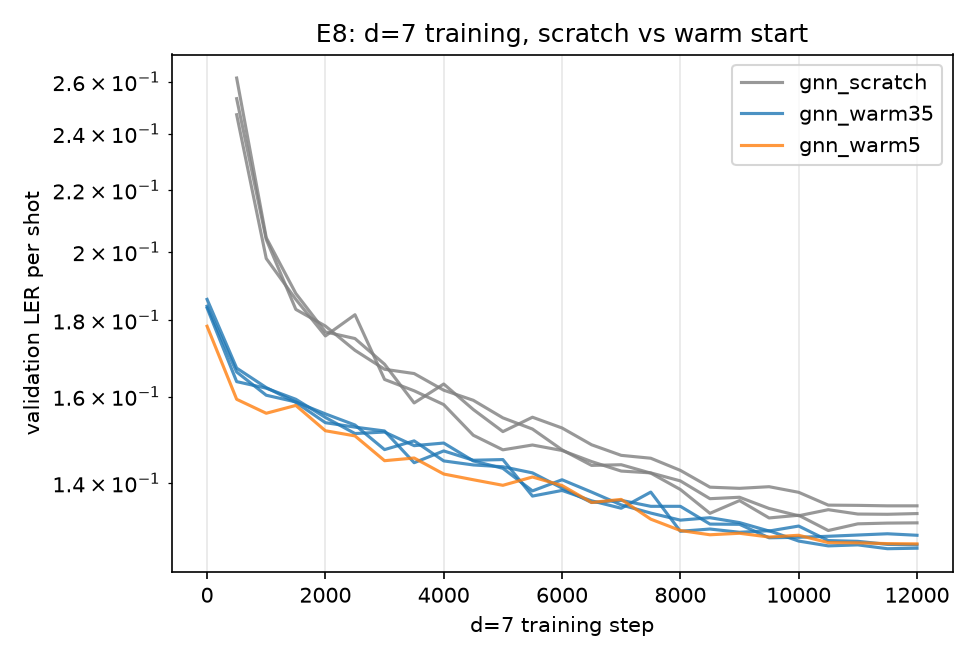
\includegraphics[width=0.66\linewidth]{e8_warmstart_curves.png}
\caption{Validation error during $d=7$ training from scratch (grey) and warm-started from $d=3,5$ (blue) or $d=5$ (orange) weights.}
\label{fig:e8}
\end{figure}
\begin{table}[t]
\centering\small
\begin{tabular}{lccc}
\toprule
$p$ & Naive MWPM & GNN from scratch & GNN warm start \\
\midrule
0.002 & $2.33\times10^{-4}$ & $(5.49\,\pm\,0.25)\times10^{-4}$ & $(4.18\,\pm\,0.09)\times10^{-4}$ \\
0.003 & $1.08\times10^{-3}$ & $(2.50\,\pm\,0.04)\times10^{-3}$ & $(2.03\,\pm\,0.04)\times10^{-3}$ \\
0.004 & $3.28\times10^{-3}$ & $(6.70\,\pm\,0.11)\times10^{-3}$ & $(5.78\,\pm\,0.10)\times10^{-3}$ \\
0.005 & $7.35\times10^{-3}$ & $(1.46\,\pm\,0.02)\times10^{-2}$ & $(1.32\,\pm\,0.01)\times10^{-2}$ \\
0.006 & $1.38\times10^{-2}$ & $(2.56\,\pm\,0.01)\times10^{-2}$ & $(2.36\,\pm\,0.01)\times10^{-2}$ \\
\bottomrule
\end{tabular}

\caption{$d=7$ test error per round: naive matching and the GNN from scratch or warm-started from $d=3,5$ weights (mean $\pm$ std over three seeds).}
\label{tab:e8}
\end{table}

\subsection{Pre-decoder}
\begin{figure}[t]
\centering
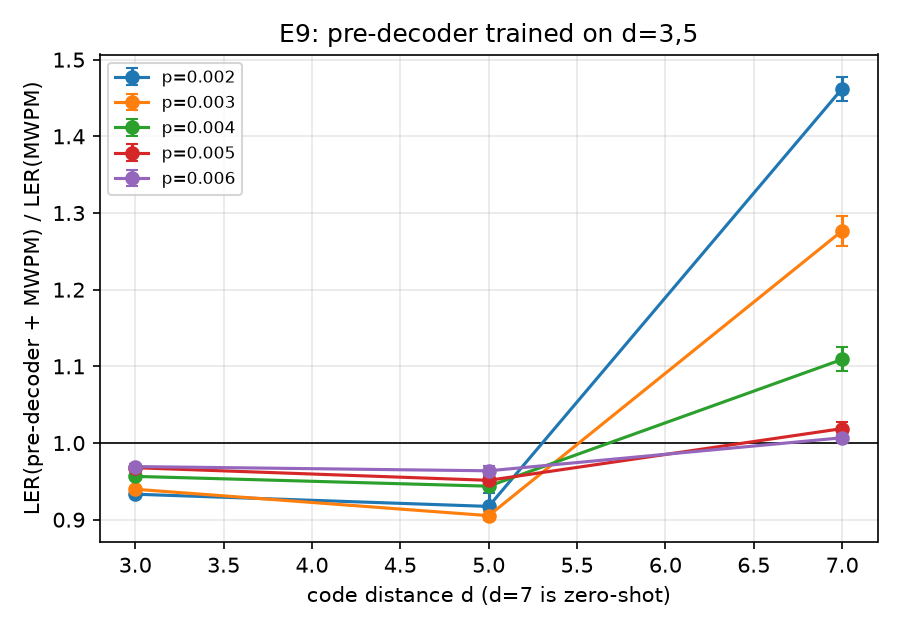
\includegraphics[width=0.48\linewidth]{e9_ratio_vs_distance.png}\hfill
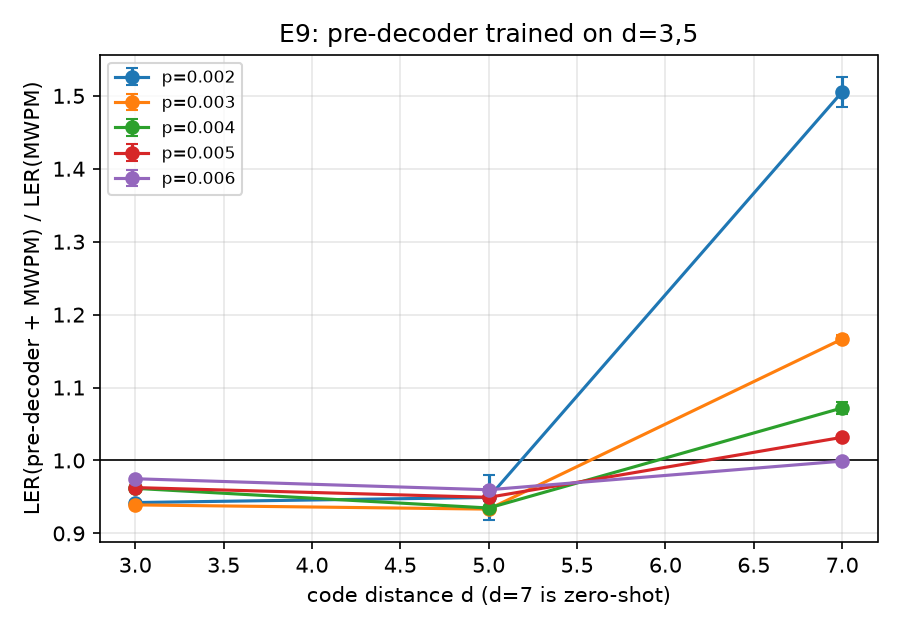
\includegraphics[width=0.48\linewidth]{e9b/e9_ratio_vs_distance.png}
\caption{Ratio of logical error rate, pre-decoder$+$matching over matching alone, on identical shots (below 1 is better). Left: $\tau=0.7$ chosen on validation shots (E9). Right: fresh-shot confirmatory test, arm A ($\tau=0.7$ again).}
\label{fig:e9}
\end{figure}
\begin{table}[t]
\centering\small
\begin{tabular}{lcccc}
\toprule
$p$ & $d=3$ & $d=5$ & $d=7$ (zero-shot) & Removed ($d=3/5/7$) \\
\midrule
0.002 & 0.933 $\pm$ 0.002 & 0.917 $\pm$ 0.017 & 1.462 $\pm$ 0.016 & 88\% / 90\% / 88\% \\
0.003 & 0.940 $\pm$ 0.003 & 0.905 $\pm$ 0.006 & 1.277 $\pm$ 0.019 & 85\% / 85\% / 83\% \\
0.004 & 0.956 $\pm$ 0.002 & 0.944 $\pm$ 0.003 & 1.109 $\pm$ 0.016 & 82\% / 81\% / 78\% \\
0.005 & 0.968 $\pm$ 0.001 & 0.951 $\pm$ 0.004 & 1.019 $\pm$ 0.008 & 79\% / 76\% / 72\% \\
0.006 & 0.969 $\pm$ 0.003 & 0.964 $\pm$ 0.006 & 1.007 $\pm$ 0.003 & 76\% / 71\% / 67\% \\
\bottomrule
\end{tabular}

\caption{Pre-decoder$+$matching over matching, $\tau=0.7$ selected on $d=5$ validation shots (mean $\pm$ std over three seeds), and the fraction of fired detectors removed. $d=7$ is zero-shot.}
\label{tab:e9}
\end{table}
At the distances it was trained on, the pre-decoder improves on matching while removing 71--90\% of fired detectors (Table~\ref{tab:e9}); at $d=3$ every paired comparison has $p<10^{-11}$, and at $d=5$ the gain is significant from $p=0.004$ upward. At $d=7$, however, the ratio grows as the error rate falls. At the verdict point ($d=7$, $p=0.002$; \nineShots{} shots, \nineErrors{} matching errors) \nineRemoved\% of fired detectors are removed, meeting the 30\% bar, but the ratio is \nineRatio, far above 1.05: the \textbf{pre-registered verdict is \emph{partial}}. A pre-decoder trained directly at $d=7$ shows the same trend (ratio $1.30$ at $p=0.002$), so this is not only a transfer failure.

\textbf{Diagnostics.} The fraction of removed faults that were truly isolated is \precMin--\precMax{} and is no lower at $d=7$ than at $d=3$; recall of isolated faults is \recMin--\recMax. A plausible explanation, which we have \emph{not} tested, is that at $d=7$ and low $p$ matching's own logical failures are so rare that a few percent of wrong removals dominate. An exploratory sweep of $\tau$ on the same test shots suggested that $\tau\ge0.95$ would pass at $d=7$, with the ratio rising above 1 only beyond roughly 70\% removal; because those shots had been seen, this could not change the verdict and needed confirmation.

\subsection{Confirmatory test}\label{sec:confirm}
\begin{figure}[t]
\centering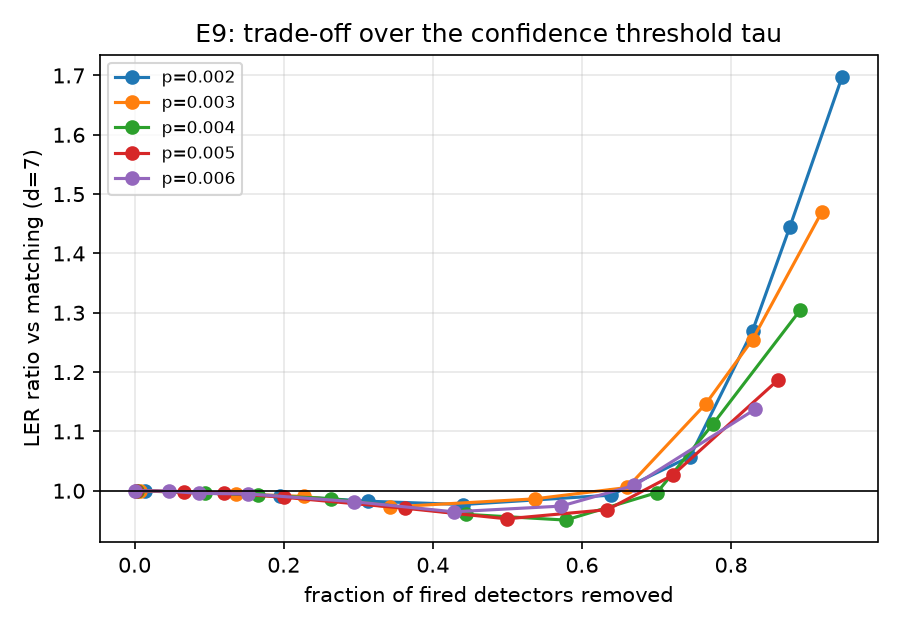
\includegraphics[width=0.66\linewidth]{e9_tradeoff_d7.png}
\caption{Exploratory threshold sweep at $d=7$ (E9 test shots): error ratio against the fraction of fired detectors removed, one curve per error rate. The ratio stays near or below 1 up to roughly 65\% removal and rises sharply beyond about 70\%.}
\label{fig:tradeoff}
\end{figure}
The confirmatory test used fresh test shots (seeds no earlier run used) and the same four trained models. Its rule was written down and committed before any of its shots were run. \textbf{Arm A} applied the pre-registered selection rule (the largest-removal $\tau$ whose ratio is at most $1.02$ at \emph{every} error rate on fresh $d=5$ validation shots); it selected $\tau'=0.7$ again, because $d=5$ validation cannot reveal the $d=7$, low-$p$ behaviour. An amendment, committed before any fresh shot, added \textbf{arm B}, a fixed $\tau=0.95$ taken from the exploratory sweep (so not selected on validation data), with the same success criterion. Table~\ref{tab:e9b} gives the results on \nineBShots{} shots with \nineBErrors{} matching errors at the verdict point.
\begin{table}[t]
\centering\small
\begin{tabular}{lcc}
\toprule
$p$ & Arm A, $\tau=0.7$ & Arm B, $\tau=0.95$ \\
\midrule
0.002 & 1.505 $\pm$ 0.021 (88\%) & 0.978 $\pm$ 0.012 (63\%) \\
0.003 & 1.166 $\pm$ 0.005 (83\%) & 0.955 $\pm$ 0.016 (53\%) \\
0.004 & 1.072 $\pm$ 0.009 (78\%) & 0.962 $\pm$ 0.003 (43\%) \\
0.005 & 1.032 $\pm$ 0.003 (72\%) & 0.978 $\pm$ 0.002 (35\%) \\
0.006 & 0.999 $\pm$ 0.002 (67\%) & 0.979 $\pm$ 0.002 (28\%) \\
\bottomrule
\end{tabular}

\caption{Confirmatory test, $d=7$ zero-shot: ratio of pre-decoder$+$matching to matching (mean $\pm$ std over three seeds) and, in parentheses, the fraction of fired detectors removed.}
\label{tab:e9b}
\end{table}
Arm A reproduced the failure (ratio \armARatio, \emph{partial}). Arm B was \textbf{positive}: ratio \armBRatio{} while removing \armBRemoved\% of fired detectors. At $p=0.002$ its difference from matching is not statistically significant (paired $p=0.07$, $0.7$ and $0.09$ across seeds); from $p=0.004$ upward all three seeds are significantly better than matching (2--4\% fewer errors). The stricter threshold has a cost: at $d=3$ the gain disappears (ratio $0.998$--$1.000$ against $0.94$--$0.975$ at $\tau=0.7$) and at $d=5$ it shrinks to $0.96$--$0.99$, so no single $\tau$ is best everywhere. A pre-decoder trained at $d=7$ reaches $0.924$ at $p=0.002$ with $\tau=0.95$.

\subsection{Latency}
\begin{table}[t]
\centering\small
\begin{tabular}{lccccc}
\toprule
$d$ & MWPM & GNN $B{=}1$ & GNN $B{=}64$ & GNN $B{=}4096$ & GNN $B{=}4096$ (GPU) \\
\midrule
3 & 1.36 & 367 & 14.8 & 4.2 & 6.3 \\
5 & 1.33 & 355 & 32.1 & 43.1 & 9.2 \\
7 & 2.03 & 271 & 38.2 & 84.5 & 7.0 \\
\bottomrule
\end{tabular}

\caption{Median microseconds per round (graph construction plus forward pass for the GNN), $p=0.004$, S0, on CPU unless stated. Hardware needs roughly 1\,$\mu$s per round.}
\label{tab:latency}
\end{table}
\begin{table}[t]
\centering\small
\begin{tabular}{lccccc}
\toprule
Setting & MWPM full & MWPM residual & Pre-dec. inference & Removal & Pre-dec. total \\
\midrule
$d=5,\ p=0.002$ & 2.1 & 0.4 & 45 & 4.0 & 49 \\
$d=5,\ p=0.004$ & 5.3 & 1.7 & 119 & 8.1 & 128 \\
$d=7,\ p=0.002$ & 6.2 & 1.7 & 184 & 11.7 & 196 \\
$d=7,\ p=0.004$ & 18.6 & 6.6 & 402 & 21.8 & 423 \\
\bottomrule
\end{tabular}

\caption{Pre-decoder timing in microseconds per shot on a CPU: matching on the full syndrome and on the residual, and the pre-decoder's own cost (inference plus the removal step).}
\label{tab:timing}
\end{table}
Matching in C++ is within a small factor of the hardware budget, while the Python GNN is two to three orders of magnitude above it (Table~\ref{tab:latency}). For the pre-decoder, matching on the residual syndrome is 3--5$\times$ faster than on the full syndrome, but the pre-decoder's own cost dominates: counting inference \emph{and} the removal step, the combination is \slowMin--\slowMax$\times$ slower than matching alone (Table~\ref{tab:timing}). This measures a Python implementation on a CPU and says nothing about a hardware realisation.

\section{Discussion}
\textbf{When does a neural decoder help?} In this benchmark, only where matching is structurally limited and the code is small. Mismatch alone is not enough, because matching can be recalibrated from syndrome data; correlated faults (crosstalk) are a genuine opening, and the GNN exploits it at $d=3,5$. Against the strongest baseline, correlated matching with the true model, the advantage is limited to $d=3$, and even there the margin is small. The GNN's data hunger (about $100\times$ calibrated matching) and its failure to scale to $d=7$ make it a weak substitute for matching as a stand-alone decoder under these budgets.

\textbf{Pre-decoders and the choice of threshold.} The pre-decoder results suggest a more promising role for neural components: remove what is easy, leave what is hard to matching. Accuracy at removal is high and does not degrade with distance, but its \emph{consequence} does. A plausible but untested explanation is that the logical failure rate of matching falls steeply with $d$ at low $p$ while an imperfect pre-decoder contributes errors at a much flatter rate. This makes the confidence threshold distance- and error-rate-dependent: a threshold validated at $d=5$ and pooled over error rates is too aggressive at $d=7$, while a stricter one is safe but forgoes the in-distribution gain. A practical pre-decoder therefore needs a threshold chosen with the target distance and error rate in mind.

\textbf{Methodology.} Two practices proved their worth. Building the calibrated and oracle baselines exposed that mismatch was a small effect, which a naive-only comparison would have hidden. And committing the protocol before the test exposed an honest failure (the first threshold) and let us confirm its fix without moving the goalposts, although the stricter threshold's origin in an earlier look at test shots means the confirmation is not fully independent.

\section{Limitations}
\begin{itemize}
\item The $d=7$ failure of the end-to-end GNN concerns this network (four layers, $\approx12$M training shots, one hyper-parameter setting) and not neural decoders in general; its validation error was still falling slowly, and one larger variant did worse.
\item The mismatch scenarios were mild (e.g.\ rate spread $\sigma=0.5$, drift $0.3$); calibrated matching nearly closes the gap by itself. Stronger or differently structured mismatch, including leakage, could favour a learned decoder; the drift experiment was inconclusive.
\item Simulated Pauli noise only; no leakage, erasure or hardware data; one code family, one memory basis, $d\le7$.
\item The strict threshold ($0.95$) was suggested by looking at earlier test shots, only one value was tested, and the pre-decoder study uses uniform noise (S0).
\item Standard deviations over three device instances or seeds are coarse, and many mismatch comparisons are within them. Test shots are not bit-identical across machines, so individual points can move by a few percent on re-running.
\item Latency was measured in Python on CPU and one GPU; it is not indicative of FPGA or ASIC performance.
\end{itemize}

\section{Conclusion}
Against calibrated and oracle matching, a syndrome-only GNN decoder gives little under mismatched noise, a modest gain under crosstalk at small distance, and does not scale to $d=7$ with this architecture and budget. A local neural pre-decoder is a more promising combination: it improves on matching where it was trained and, with a sufficiently conservative threshold, transfers to $d=7$ on fresh shots while removing most of matching's input, though its Python implementation is not yet faster than matching. The harder questions are left open: whether larger receptive fields or longer training rescue the end-to-end network, how to choose the threshold without knowing the target distance, and whether the pre-decoder helps under correlated noise and on hardware.

\section*{Reproducibility and data availability}
All code, per-point and per-shot results, figures and one record per run (environment, commit, configuration, test results and every metric) are in the project repository, with commands to regenerate every table and figure; the tables in this paper are generated from the stored results by a script. Trained checkpoints are small but not committed. Compute used: about four hours of one RTX 4090 for the GNN experiments, under one hour for each of the warm-start and pre-decoder trainings, and a local CPU for all evaluation. The pre-registration of the pre-decoder study and its amendment are in the repository's design document, committed before the corresponding shots were run.

\begin{thebibliography}{99}\small
\bibitem{dennis2002} E.~Dennis, A.~Kitaev, A.~Landahl, J.~Preskill. Topological quantum memory. \emph{J. Math. Phys.} 43, 4452 (2002).
\bibitem{fowler2012} A.~G.~Fowler, M.~Mariantoni, J.~M.~Martinis, A.~N.~Cleland. Surface codes: towards practical large-scale quantum computation. \emph{Phys. Rev. A} 86, 032324 (2012).
\bibitem{fowler2015} A.~G.~Fowler. Minimum weight perfect matching of fault-tolerant topological quantum error correction in average $O(1)$ parallel time. \emph{Quantum Inf. Comput.} 15, 145 (2015).
\bibitem{higgott2022} O.~Higgott. PyMatching: a Python package for decoding quantum codes with minimum-weight perfect matching. \emph{ACM Trans. Quantum Comput.} 3, 16 (2022).
\bibitem{higgott2023sparse} O.~Higgott, C.~Gidney. Sparse Blossom: correcting a million errors per core second with minimum-weight matching. arXiv:2303.15933 (2023).
\bibitem{higgott2023belief} O.~Higgott, T.~C.~Bohdanowicz, A.~Kubica, S.~T.~Flammia, E.~T.~Campbell. Improved decoding of circuit noise and fragile boundaries of tailored surface codes. \emph{Phys. Rev. X} 13, 031007 (2023).
\bibitem{gidney2021stim} C.~Gidney. Stim: a fast stabilizer circuit simulator. \emph{Quantum} 5, 497 (2021).
\bibitem{gidney2021honeycomb} C.~Gidney, M.~Newman, A.~Fowler, M.~Broughton. A fault-tolerant honeycomb memory. \emph{Quantum} 5, 605 (2021).
\bibitem{torlai2017} G.~Torlai, R.~G.~Melko. Neural decoder for topological codes. \emph{Phys. Rev. Lett.} 119, 030501 (2017).
\bibitem{bausch2024} J.~Bausch \emph{et al.} Learning high-accuracy error decoding for quantum processors. \emph{Nature} 635, 834 (2024).
\bibitem{lange2025} M.~Lange \emph{et al.} Data-driven decoding of quantum error correcting codes using graph neural networks. \emph{Phys. Rev. Research} 7, 023181 (2025).
\bibitem{delfosse2020} N.~Delfosse. Hierarchical decoding to reduce hardware requirements for quantum computing. arXiv:2001.11427 (2020).
\bibitem{chamberland2023} C.~Chamberland, L.~Goncalves, P.~Sivarajah, E.~Peterson, S.~Grimberg. Techniques for combining fast local decoders with global decoders under circuit-level noise. \emph{Quantum Sci. Technol.} 8, 045011 (2023).
\end{thebibliography}
\end{document}
